\documentclass[brudnopis]{xmgr}
\usepackage{listings}
\setmainfont[Numbers=OldStyle,Mapping=tex-text]{Minion Pro}
\setsansfont[Numbers=OldStyle,Mapping=tex-text]{Myriad Pro}

\wersja   {wersja wstępna [\ymdtoday]}

\author   {Wojciech Denejko}
\nralbumu {214\,300}
\email    {deneyw@gmail.com}

\title    {Rozpoznawanie tekstu w aplikacjach mobilnych}
\date     {2017}
\miejsce  {Gdańsk}

\opiekun  {dr Tomasz Borzyszkowski}

\begin{document}

% streszczenie
\begin{abstract}
  Niniejsza praca ma na celu stworzenie aplikacji rozpoznającej tekst w języku polskim oraz angielskim, charakteryzująca się kompatybilnością z systemami iOS oraz Android. Do wytworzenia aplikacji zostanie użyta platforma Xamarin, która służy do tworzenia aplikacji wieloplatformowych. Zbadane zostaną różne metody połączenia technologi wieloplatformowej z istniejącymi rozwiązaniami OCR. Przedstawiona konwolucyjna sieć neuronowa zaprezentuje klasyfikacje polskiego alfabetu.
  
  Integralną częścią pracy będzie aplikacja OCRecognizer, w której zaimplementowano metody klasyfikacji obrazów. Program umożliwia zrobienie zdjęcia, a następnie przy użyciu kilku opcji, rozpoznanie tekstu.
  
\end{abstract}

% słowa kluczowe
\keywords{C\#,
 Xamarin,
 .NET,
 Uczenie maszynowe,
 Sieci neuronowe,
 kNN,
 }

% tytuł i spis treści
\maketitle

% wstęp
\introduction

	Xamarin to platforma deweloperska służąca do tworzenia natywnych aplikacji mobilnych dla systemów iOS, Android oraz Windows, za pomocą wspólnej technologii .NET i języka C\# . Dzięki temu możliwe jest uzyskanie do stu procent wspólnego kodu między różnymi platformami. Aplikacje napisane przy użyciu technologii Xamarin i C\# mają pełny dostęp do interfejsów, API oraz możliwość tworzenia natywnych interfejsów użytkownika.
  
  Ze względu na dynamiczny rozwój rynku IT, uczenie maszynowe staje się coraz bardziej popularne a algorytmy zyskują lepszą skuteczność dzięki dostępności danych oraz szybszych podzespołów komputerowych. 
  
  Urządzenia przenośne mają stosunkowo ograniczone zasoby w związku z tym istnieje problem powiązania tych dwóch dziedzin. Algorytmy systemów uczących się wymagają dużej mocy obliczeniowej. Aplikacje wieloplatformowe pozwalają zaoszczędzić czas na implementacji oraz skuteczniej tworzyć funkcjonalności rozpoznawania tekstu. Połączenie tej technologi z algorytmem służącym do klasyfikacji znaków w obrazie jest bardziej optymalne niż ich natywne odpowiedniki.
  
  Celem pracy jest  zbadanie istniejących rozwiązań służących do rozpoznawania tekstu oraz stworzenie sieci neuronowej pozwalającej na klasyfikację znaków pisanych charakterystycznych dla współczesnego języka polskiego. Ponieważ pozyskanie danych z polskimi znakami potrzebnych do trenowania sieci neuronowej stanowi problem, zostało stworzone narzędzie do odczytywania znaków z kartki papieru, a następnie zapisanie ich w formie obrazu 32x32 piksele, w skali szarości.

\chapter{Rozpoznawanie tekstu w aplikacjach wieloplatformowych}

OCR (ang. Optical Character Recognition) jest to technika lub część oprogramowania służąca do rozpoznawania znaków oraz całych tekstów w pliku graficznym prezentowanym za pomocą pionowo-poziomej siatki odpowiednio kolorowanych pikseli. Przykładem takiej grafiki jest zdjęcie z aparatu cyfrowego. 

Niegdyś pojęcie rozpoznawania znaków oznaczało samą klasyfikacje ciągów znaków drukowanych, które są łatwiejszym problemem do rozwiązania, dziś również pisma odręczne oraz cechy formatowania, takie jak krój pisma, stopień pisma lub układy tabelaryczne (formularze).

Techniki OCR głównie wykorzystawane są do cyfryzacji zasobów bibliotek, a także jako ułatwienie przy odczytywaniu dokumentacji napisanych pismem odręcznym, w aplikacjach mobilnych rozpoznawanie znaków pomaga w takich zadaniach jak tworzenie notatek, a następnie tłumaczenie ich na tekst drukowany. Niestety, w obu przypadkach istniejące rozwiązania OCR nie są tak skuteczne jak człowiek, zatem w przypadkach trudności z klasyfikacją znaku lub fragmentu tekstu niezbędna jest weryfikacja wyniku przez człowieka celem uniknięcia błędu.

Postęp w metodach OCR jest bardzo widoczny gdyż w obecnych czasach produkty potrafią rozpoznawać mało dokładne skany, wykonane telefonami komórkowymi z szumami na obrazkach, z tekstem napisanym pod nienaturalnymi kątami w wielu językach, pozostaje jednak problem rozpoznawania znaków pisma odęcznego.

Rozpoznawanie pisma jest możliwe dzięki zastosowaniu metod z dziedziny rozpoznawania wzorców, czyli pola badawczego w obrębie uczenia maszynowego. Metoda ta może być definiowana jako działanie polegające na pobieraniu danych i podejmowaniu dalszych czynności zależnych od kategorii do której należą te dane. By odpowiednio wyodrębnić poszczególne znaki z obrazu używane są biblioteki pozwalające na profesjonalną obróbkę zdjęć pod zastosowania w celach uczenia maszynowego. Przykładem takiej biblioteki jest OpenCV. Następnie po wyodrębnieniu potrzebnych informacji na temat danego znaku obrazy są klasyfikowane jako poszczególne litery. Zwykle w tym procesie używane są sieci neuronowe.

Kompletny system rozpoznawania wzorców składa się z:
\begin{itemize}
\item
zbioru danych, które oferują możliwość klasyfikacji lub opisu
\item
mechanizmu wydobywania cech, które najlepiej charakteryzują i separują daną klase, do której dany element zbioru danych należy
\item
mechanizmu przekształcenia elementu zbioru w symboliczną informacje, łatwiejszą do wykorzystania przez algorytm
\item
schematu decyzyjnego lub schematu opisu, który realizuje właściwą część procesu klasyfikacji w oparciu o wydobyte i przekształcone cechy obiektu.
\end{itemize}

\section{Przedstawienie problemu}

Wsród istniejących rozwiązań mogących służyć jako narzędzie potrzebne do wytworzenia aplikacji mobilnej, która rozpozna polskie znaki pisma odręcznego nie istnieje łatwy sposób zastosowania rozwiązania pozwalającego na skuteczną klasyfikacje polskiego pisma. Brakuje również dostępnych danych wymaganych do skutecznej klasyfikacji w oparciu o przekształcone informacje. Aby rozwiązać ten problem należy stworzyć zbiór treningowy lub rozszerzenie istniejącego zbioru danych o polskie znaki alfabetu.

Dostępne biblioteki na rynku, takie jak TesseractAPI oraz Microsoft Computer Vision API oferują wysoką skuteczność w rozpoznawaniu polskich oraz angielskich obrazów tekstu drukowanego lecz zarazem brak możliwości rozpoznawania pisma odręcznego. Wymagane jest więc stworzenie systemu rozpoznawania wzorców, który pozwalałby na skuteczną klasyfikacje znaków pisma odręcznego.

Kolejnym problemem są znacząco ograniczone zasoby urządzeń mobilnych. Systemy rozpoznawania wzorców wymagają mocy obliczeniowej potrzebnej do przekształcenia obrazów w postać pozwalającą na wyodrebnienie cech, a następnie przeprowadzenie procesu klasyfikacji. Rozwiązaniem tego problemu jest wykorzystanie systemu rozpoznawania wzorców jako serwisu internetowego działającego w oparciu o architekture REST.

\section{Sposób wytworzenia zbioru treningowego}

Zbiór treningowy jest kontenerem krotek (przykładów, obserwacji, próbek), będących lista właściwości atrybutów opisowych (tzw. deskryptorów) i wybranego atrybutu decyzyjnego (ang. class label attribute). Głównym jego celem jest zbudowanie formalnego modelu zwanego klasyfikatorem. Wynikiem procesu klasyfikacji jest pewien otrzymany model (klasyfikator), który przydziela każdemu przykładowi wartość atrybutu decyzyjnego w oparciu o właściwości pozostałych atrybutów.

W przypadku systemu rozpoznawania wzorów zbiorem treningowym są zdjęcia obrazów zawierajace odpowiednio wszystkie litery polskiego alfabetu oraz cyfry. Wszystkie zdjęcia liter, które istnieją w zbiorze należy przeformatować do postaci najlepiej rozumianą przez wykorzystywane algorytmy.

Do transformacji zdjęć zastosowano EmguCV, jest to wieloplatformowa implementacja (ang. wrapper) w technologi .NET biblioteki OpenCV, pozwalająca na wykorzystanie funkcjonalności OpenCV w środowisku .NET we wszystkich jego językach programowania takich jak C\#, VB, F\#. Można ją zainstalować używając menadżera pakietów Nuget w programie Visual Sutdio, Xamarin Studio lub Unity, a więc jest również kompatybilna z platformami mobilnymi Android oraz iOS.

Transformacja zdjęcia przebiega następująco:
\begin{itemize}
\item
Odczytaj zdjęcie w formacie .png
\item
Przeprowadź konwersje kolorów RGB na odcienie szarości
\item
Przetwórz obraz do formatu 28 x 28 pikseli
\item
Odczytaj stopień jasności każdego piksela w skali od 0 do 255 i zapisz je w tablicy
\end{itemize}

\begin{figure}[!tbh]
\centering
\includegraphics[width=.6\hsize]{fig/ą}
\caption{Przykład zdjęcia znaku}
\end{figure}
Rezultatem działania programu do konwersji zdjęć jest plik train.csv. Zawiera ona 785 kolumn. Pierwsza kolumna, nazwana "label", określa znak, który jest narysowany. Reszta kolumn zawiera informacje na temat jasności każdego piksela.

Każda kolumna w zbiorze treningowym ma ustawioną nazwę pixelx, gdzie x jest liczbą między 0 a 783. By znaleźć dany piksel na obrazie, należy rozłożyć x jako x = a * 28 + b, gdzie a i b to liczby między 0 a 27. Wtedy pixelx jest umieszczony w a-tym rzędzie b-tej kolumnie w macierzy 28 x 28, indeksowanej od zera. Na przykład, pixel31 wskazuje na to, piksel w czwartej kolumnie od lewej i drugim wierszu od góry. Tak jak pokazane na diagramie poniżej:

\begin{lstlisting}
000 001 002 003 ... 026 027
028 029 030 031 ... 054 055
 |   |   |   |  ...  |   |
728 729 730 731 ... 754 755
756 757 758 759 ... 782 783 
\end{lstlisting} 

Aplikacją generującą zbiór treningowy jest program TrainingSetGenerator, kod przeprowadzający transformacje oraz komentarze załączony jest poniżej:

// kod

\section{Algorytm k-NN}

Algorytm k-najbliższych sąsiadów (ang. k nearest neighbours) - algorytm regresji nieparametrycznej najczęściej używany w statystyce do prognozowania pewnej wartości zmiennej losowe.

Założenia:
\begin{itemize}
\item
Dany jest zbiór teningowy, który stworzony został w oparciu o narzędzie TraningSetGenerator.
\item
Dana jest obserwacja C, zawierająca wektor zmiennych pixel0 ... pixel783, dla której chcemy prognozować wartość zmiennej objaśnianej label.
\end{itemize}	

   Ilustracja przedstawiająca przykład działania algorytmu k najbliższych sąsiadów:

Algorytm działa następująco:
\begin{itemize}
\item
Porównaj wartości zmiennych objaśniających dla obserwacji C, z każdym wektorem w zbiorze treningowy.
\item
Wyborze k (ustalonej z góry liczby) najbliższych do C obserwacji ze zbioru treningowego.
\item
Uśrednieniu wartości zmiennej objaśnianej dla wybranych obserwacji, w wyniku czego uzyskujemy prognozę.	
\end{itemize}	
     
\begin{figure}[!tbh]
\centering
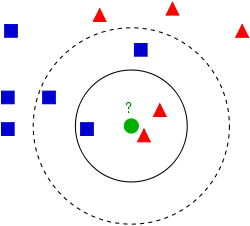
\includegraphics[width=.6\hsize]{fig/knn}
\caption{Przykład problemu k-NN}
\end{figure}
\newpage
Dla k = 3, niewiadoma oznaczona zielonym punktem będzie sklasyfikowana jako czerwony trójkąt w oparciu o trzech najbliższych sąsiadów, jednak jeśli k = 5, zostałaby sklasyfikowana jako niebieski kwadrat ponieważ algorytm działałby w oparciu o pięciu sąsiadów. Najbliżsi sąsiedzi są określani przy pomocy metryki euklidesowej określonej wzorem:

\begin{figure}[!tbh]
\centering
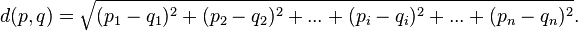
\includegraphics[width=.8\hsize]{fig/knn-wzor}
\end{figure}

// kod

\section{Random Forest}

Algorytm Random Forest to metoda klasyfikacji polegająca na tworzeniu wielu drzew decyzyjnych na podstawie zestawu danych. Idea tego klasyfikatora polega na zbudowaniu zgromadzeniu najlepszych z losowych drzew decyzyjnych, w klasycznych drzewach decyzji, losowe drzewa budowane są na zasadzie podzbiorów analizowanych cech w węźle, które dobierane są losowo.

Cechy algorytmu Random Forest:
\begin{itemize}
\item
działa skutecznie na dużych zbiorach treningowych
\item
utrzymuje dokładność w przypadku gdy dane są nie kompletne lub jest ich mało
\item
daje oszacowanie, które zmienne są istotne w klasyfikacji
\item
lasy drzew mogą być zapisane i wykorzystane w przyszłości dla innego zbioru danych
\item
nie jest podany na przeuczenie (ang. overfitting)
\end{itemize}

Algorytm działa następująco:
\begin{itemize}
\item
Losujemy ze zwracaniem z n-elementowego zbioru treningowego n wektorów. Na podstawie takiej próby zostanie stworzone drzewo.
\item
W każdym węźle podział odbywa się poprzez wylosowanie bez zwracania m spośród p atrybutów, następnie w kolejnym węźle k spośród m atrybutów
\item
Proces budowania drzewa bez przycinania trwa, jeśli to możliwe do momentu uzyskania w liściach elementów z tylko jednej klasy.
\end{itemize}

Proces klasyfikacji:
\begin{itemize}
\item
Dany wektor obserwacji jest klasyfikowany przez wszystkie drzewa, ostatecznie zaklasyfikowany do klasy, w której wystąpił najczęściej.
\item
W przypadku elementów niewylosowanych z oryginalnej podpróby, każdy taki i-ty element zostaje poddany klasyfikacji przez drzewa, w których budowie nie brał udziału. Taki element zostaje następnie przyporządkowany klasie, która osiągana była najczęściej.
\end{itemize}

\begin{figure}[!tbh]
\centering
\includegraphics[width=.6\hsize]{fig/randomforest}
\caption{Diagram przepływu algorytmu Random Forest}
\end{figure}
\newpage

//kod

\section{Jednokierunkowe, dwuwarstwowa sieć neuronowe}

Siecią neuronową nazywa się programową lub sprzetową strukturę modeli, realizujaca obliczenia lub przetwarzajaca sygnały poprzez rzędy elementów, zwanych sztucznymi neuronami. Emulują one niektóre spośród zaobserwowanych właściwości biologicznych układów nerwowych. Sztuczne sieci neuronowe są swoistym systemem inspirowanym przez to, w jaki sposób gesto połączone między sobą struktury mózgu, odbierają i przetwarzają dane które docierają w różny sposób z otoczenia. Kluczowytm elementem jest zatem struktura systemu przetwarzania informacji. Sieć taka sklada sie z dużej liczby rozlegle połączonych ze sobą elementów przetwarzajacych, które są powiazane ze sobą ważonymi połaczeniami.

Cechą charakterystyczna sieci neuronowych od algorytmów realizujacych przetwarzanie informacji przy użyciu algorytmów jest umiejetność generalizacji, czyli zdolność uógolniania wiedzy dla nieznanych wczesniej wzorców. Innym atutem jest także zdolność do aproksymacji wartości funkcji wielu zmiennych w przeciwienstwie do interpolacji, która jest możliwa do uzyskania używając przetwarzania algorytmicznego.

Uczenie sieci neronowych zmienia liczbowe wartości wag znajdujacych się pomiędzy neuronami. Nastepuje to poprzez bezposrednią ekspozycje rzeczywistego zestawu danych, gdzie algorytm uczący modeluje wagi polaczeń. Ze względu na opisane powyżej cechy i zalety, obszar zastosowań sieci neuronowych jest rozlegly:

\begin{itemize}
\item
Rozpoznawanie wzorców
\item
Klasyfikowanie obiektów
\item
Prognozowanie i ocena ryzyka ekonomicznego
\item
Prognozowanie zmian cen rynkowych
\item
Ocena zdolności kredytowej
\item
Ocena wniosków ubezpieczeniowych
\item
Rozpoznawanie wzorów podpisów
\item
Diagnostyka medyczna
\item
Prognozowanie sprzedaży
\item
Analizowanie zachowań klienta w supermarketach
\end{itemize}

Podstawowym elementem sieci neuronowej jest neuron. Jego schemat zostal opracowany przez McCullocha i Pittsa w roku 1943, zostal on oparty na budowie biologicznej komorki nerwowej.

// schemat sztucznego neuronu.

Do wejsc doprowadze sa sygnaly z wejsc sieci lub neuronow warstwy poprzedniej. Kazdy sygnal mnozony jest przez odpowiadajaca mu wartosc liczbowa zwana waga. Wplywa ona na percepcje danego sygnalu wejsciowego i jego udzial w sygnale wyjsciowym przez neuron. Waga moze byc dodania lub ujemna, jezeli nie ma polaczenia miedzy neuronami to waga jest rowna zero. Zsumowane iloczyny wag i sygnalow sa argumentem funkcji zwanej funkcja aktywacji neuronu.

Wartość funkcji aktywacji jest wyjściem neurona i propagowana jest do neuronów warstwy następnej. Może ona przybierać jedną z trzech postaci:
\begin{itemize}
\item
- nieliniowa
\item
- liniowa
\item
- skoku jednostkowego
\end{itemize}

Należy zauważyć, iż jest to podział bardziej formalny niż merytoryczny. Różnice funkcjonalne między tymi typami raczej nie występują, natomiast można stosować je naprzemiennie w różnych warstwach sieci.

Najbardziej popularnym typem sieci neuronowej jest sieć wielowarstwowa (ang. Multi-Layer Neural Network). Jej cecha charakterystyczna jest wystepowanie co najmniej jednej warstwy ukrytej neuronow, posredniczacej w przekazywaniu sygnalow pomiedzy wejsciami a wyjsciami sieci.

// schemat budowy sieci wielowarstwowej

Do rozpoznania polskich znakow pisma odrecznego uzyta zostala siec posiadajaca trzy warstwy.

// schemat sieci

Warstwa wejsciowa sieci sklada sie z neuronow zawierajacych informacje na temat kazdego piksela. Zbior treningowy sklada sie z obrazow 28 x 28 pikseli. Zgodnie z tym zalozeniem pierwsza warstwa sieci bedzie skladala sie z 784 neuronow. Kazdy neuron przechowuje wartosc skali szarosci piksela, gdzie 0.0 oznacza kolor bialy, a 1.0 czarny.

Druga warstwa zawiera liczbe n neuronow, liczba n jest uzywana w kontekscie eksperymentalnym.

Ostatnia warstwa, zawiera 74 neurony, poniewaz w Polski alfabet sklada sie z 32 liter, rozpatrywane sa zarowno litery wielkie jak i male oraz cyfry. Implementacja sieci:

// kod

\section{Konwolucyjne sieci neuronowe - CNN}

Konwolucyjne sieci neuronowe (ang. Convolutional Neural Networks) sa podobne do klasycznych sieci neuronowych. Aby dokladnie przeanalizowac budowe oraz dzialanie CNN przedstawiony zostanie problem klasyfikacji dwoch liter X i O. Ten przyklad demonstruje charakterystyczne reguly konwolucji.

// x ?= X

CNN porownuje obrazy w kawalkach. Kazda taka czesc nazywana jest cecha (ang. feature), nastepnie oba zdjecia przeszukiwane sa na podobnych pozycjach by uzyskac jak najwiecej cech wspolnych. Sieci konwolucyjne duzo lepiej wspolpracuja na podobienstwach niz na pracy z pelnym obrazem, ktory pasuje do pewnego wzorca.

// x features

Kazda ceche mozna scharakteryzowac jako mniejsze zdjecie - dwuwymiarowa tablice wartosci. W przypadku litery X, cechami beda ukosne linie i znak krzyza, w ten sposob uzyskuje sie cechy charakterystyczne danego znaku.

// features zdjecie



\section{Podsumowanie}

\chapter{Implementacja aplikacji do rozpoznawania tekstu}

\section{Xamarin.Android i Xamarin.iOS}

\section{Xamarin.Forms}

\section{Microsoft Computer Vision API}

\section{Microsoft Azure for Machine Learning}

\section{Tensorflow}

\chapter{Metryki oraz testy}

\section{Testy wydajnościowe}

\section{Testy zgodności}

\section{Testy użyteczności}

\section{Cross Validation}

\section{Macierze błędu}

\section{Metryki wyliczane z kodu źródłowego}

\section{Macierze wyliczane z diagramów}

\section{Macierze pomiaru wspólnego kodu}

\chapter{Podsumowanie i wnioski}

\section{Wady oraz zalety aplikacji wieloplatformowych}

\section{Uczenie maszynowe w aplikacjach mobilnych}

\section{Koszt}

% zakończenie
\summary

% literatura (obowiązkowo):
\bibliographystyle{unsrt}
\bibliography{xml}

\oswiadczenie

\end{document}